%!TEX encoding = UTF-8 Unicode
% XeLaTeX can use any Mac OS X font. See the setromanfont command below.
% Input to XeLaTeX is full Unicode, so Unicode characters can be typed directly into the source.

% The next lines tell TeXShop to typeset with xelatex, and to open and save the source with Unicode encoding.
%!TEX TS-program = xelatex 

\documentclass[a4paper, 12pt]{book}
%Load FDU Style
\usepackage{FDUThesis}
\usepackage{mathrsfs}
\usepackage{siunitx}
%\usepackage{wordcount}
%\usepackage{vector}
\usepackage{float}
\usepackage{graphicx}
\usepackage{amsmath}
\usepackage{amssymb}
\usepackage{grffile} %Prevent the file path of an image appearing above the image
%\usepackage[utf8]{inputenc}
%\usepackage[T1]{fontenc}
\usepackage{textcomp}
\usepackage{gensymb}
\usepackage{mathtools}  % to input small matrix 
\usepackage{placeins} % prevent the graph to float to another section \FloatBarrier

\newcommand{\bvec}{\mathbf}
\graphicspath{{./Pic/},{./Pic/OTS/},{./Pic/PumpRepump/},{./Pic/Parafin/},{./Pic/chapter2/},{./Pic/chapter3/},{./Pic/Intro/}} 
 
\title{Wang Mengbing's Article} 
\author{Wang Mengbing $<$\href{mailto:menbinwan@gmail.com}%
            {menbinwan@gmail.com}$>$}
  
%\date{}                                         % Activate to display a given date or no date

\begin{document}
%Use \thispagestyle{} fancy, plain, empty to redefine Per/Page Header

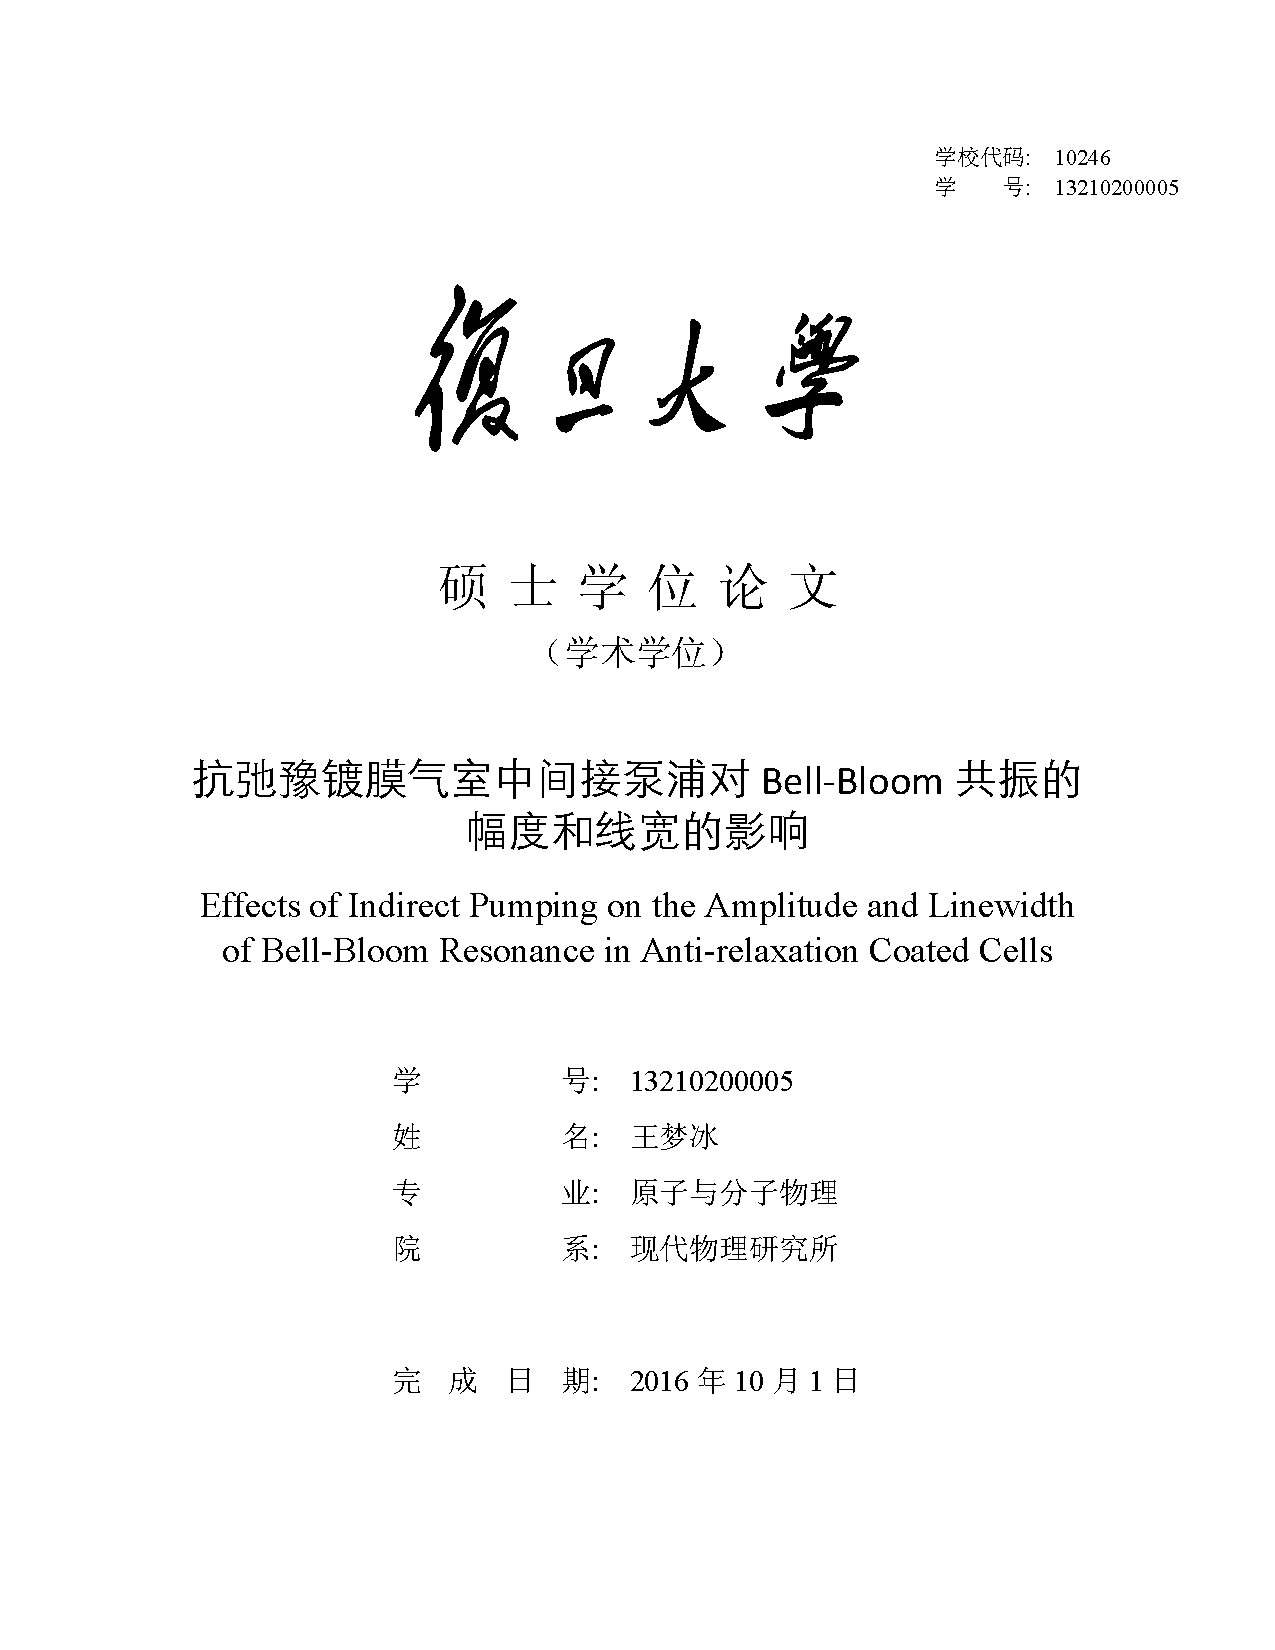
\includepdf{Book-Cover.pdf}
\thispagestyle{empty}
%----------------------------Front Matter-------------------------------!
\frontmatter
%\maketitle

\phantomsection
\addcontentsline{toc}{chapter}{\contentsname}
\tableofcontents

%{\pagestyle{plain}
%\tableofcontents
%\cleardoublepage}



\frontchapter{评审委员会}

\frontchapter{中文摘要}
\iffalse
原子磁力仪在测量时间为$T$,测量原子数为$N$,相干时间为$\tau$时的灵敏度为$\delta B=\frac{1}{g \mu_B}\frac{\hbar}{\sqrt{N \tau T}}$。其中$\mu_B$为玻尔磁子,$g$为基态的朗德$g$因子,$\hbar$为普朗克常数。增大基态的相干时间$\tau$的方法是减少弛豫,如壁弛豫,自旋碰撞弛豫等。在磁力仪信号上的表现则为更大的信号幅度和更小的展宽。
\fi
本文首先对双共振磁力仪和Bell-Bloom磁力仪的线型展开解析和数值计算,分别用到极化矢量模型和密度矩阵方法。计算结果表明,在两种磁力仪中,直接泵浦光都会产生功率展宽;在不考虑壁弛豫和自旋碰撞弛豫,而仅仅假设一个各项同性的弛豫机制下,间接泵浦光都不会产生功率展宽。本文的第二部分为实验研究,我们比较了OTS和石蜡气室中,在相同条件下,以及在同一气室中不同自旋交换速率下,间接泵浦对Bell-Bloom线宽和振幅的影响,并发现间接泵浦造成的功率展宽比直接泵浦小两个数量级,且信号幅度相当。另外间接泵浦功率展宽来自于壁碰撞或自旋交换碰撞对不同超精细能级上自旋去相干的传递。

\iffalse
我们在镀有OTS和石蜡抗弛豫镀膜的气室中,在不同温度下,即不同自旋交换碰撞率下,对Bell-Bloom磁力仪的线型进行详细研究。从实验结果上推测间接泵浦过程中泵浦光会通过自旋交换碰撞和壁碰撞传递功率展宽,且其引起的展宽相比直接泵浦小约两个数量级。
\fi

\bigskip
\noindent \textbf{关键词:\hspace{\Han}}
间接泵浦,Bell-Bloom磁力仪,功率展宽,自旋交换碰撞,壁弛豫

\bigskip
\noindent \textbf{中图分类号:\hspace{\Han}}
\frontchapter{Abstract}
In this thesis, we first derived the linewidth of the double resonance magnetometry using the polarization model and the density matrix method, analitically and numerically. We found no power-broadening effect from the indirect pumping light in both double resonance and Bell-Bloom magnetometry if ignoring effects of the wall and spin-exchange relaxation and assuming only isotropic relaxation process. In the second part of this thesis, we investigated the effect of indirect pumping on the lineshape of Bell-Bloom resonance in OTS and paraffin coated cells under the same condition, and at different spin exchange rates in the same cell. And found that the powerbroadening from the indirect pumping light is two orders of magnitude than that of the direct pumping with the comparable amplitude. The power broadening of indirect pumping light comes from the transfer of spin decoherence between different hyperfine levels.  
\iffalse
The sensitivity of a magnetic-field measurement for a magnetomery performed for a time $T$ with an ensemble of $N$ atoms with coherence time $\tau$ is $\delta B=\frac{1}{g \mu_B}\frac{\hbar}{\sqrt{N \tau T}}$, where $\mu_B$ is the Bohr magneton, g is the ground-state Landé factor, and $\hbar$ is Planck’s constant. To increase the coherence time $\tau$, one has to reduce the relaxation of polarization including the wall relaxation, spin-exchange relaxation and so on. So a larger amplitude of Lorentz signal with narrower linewidth is observed.
\fi

\bigskip
\noindent  \textbf{Key Words:\hspace{\Han}}
Indirect Pumping, Bell-Bloom Magnetometry, Power Broadening, Spin-exchange Collisions, Wall Relaxation

\bigskip
\noindent \textbf{CLC Number:\hspace{\Han}  }



%\listoffigures
%\listoftables

%----------------------------Main Matter-------------------------------!
\mainmatter


%\include{Intro}

%\include{Chapter01}

%\include{Chapter02}

%\include{Chapter03}

%\include{Chapter04}
\input{Chapters/Intro}

\input{Chapters/Chapter1} % Introduction and background theory

\input{Chapters/Chapter2} % Calculation Method and Result

\input{Chapters/Chapter3} % Experiment Data and Analysis

\input{Chapters/publishing}
%----------------------------Appendix-------------------------------!
\appendix  

\renewcommand{\thechapter}{附录{\Alph{chapter}}}

%\chapter{公式推导}
%----------------------------Back Matter-------------------------------!
\backmatter{}

\phantomsection
\addcontentsline{toc}{chapter}{\bibname}
\bibliographystyle{FDUbib}
\bibliography{Bibliography}
%\nocite{*}

\backchapter{致谢}



感谢赵凯锋导师指导,特别是最后阶段对论文和答辩报告幻灯片提出的修改意见。感谢王美玲师姐在我刚来实验室时的帮助,特别是在我研一时候组织的激光物理读书会开启了科研的大门。也感谢魏丽花师姐,优美的歌声不会忘记。在和廖康佳师兄对物理问题的讨论中,他独到的见解经常让我有超出预期的收获。感谢张桂迎师兄,他大量的文献阅读量使得在和他的讨论中,能够得知许多工作组目前在做的工作方向和最新进展,推荐文献以供学习研究。并且在生活中也给我许多指导。

感谢我在研究生阶段初期选课期间给我们授课的物理系各位老师,以及在课堂上认识的同学们。老师知识渊博,对于教学有着自己的思路和方式,非常真诚,做出了许多工作让学生尽可能多的理解;有幸认识了一群真正喜欢物理,并愿意做物理的同学们。在观察他们与老师的讨论中和与他们的讨论中,感受到执着和智慧,对待知识精益求精。

这里特别感谢徐建军老师,有幸选修徐老师的几门课,在他的引导下与和同班许多同学的讨论中好好学了两门课,感到自己进步好多,对物理的感觉建立起来。同样需要特别感谢吴赛骏老师,让我看到一流科研工作者的科研精神和风貌,实验室外的交流中学到了课本上不会讲的学习方法和感悟,回答了长期困扰自己的许多问题,让我有醍醐灌顶的感觉。

感谢现代物理研究所的每一位同学,每个同学身上都有闪光点,让我知道自己的不足和努力方向;

如果复旦是形容词,那么一定可以用来形容他们。

感谢现代物理研究所的杨明杰老师、杨柳老师、封娅娅老师、王冕老师及査老师对我毕业办理手续过程中提供的支持和帮助。感谢其他老师让我加快成长的速度,增长了我的阅历和见识。

最后感谢自己的父母,前十八年你们的养育工作已经顺利完成,剩下一棒就交给我自己了。

\clearpage
\printindex
\end{document}
